\documentclass[a4paper, titlepage, 10pt]{book}


\usepackage{graphicx}
\usepackage{caption}
\usepackage{amsmath,amssymb}
\usepackage{siunitx}
\usepackage{hyperref}

%impostazioni pagina
\usepackage{geometry}
\geometry{a4paper, top=2.5cm, bottom=2.5cm, left=2.4cm, right=2.4cm, heightrounded, bindingoffset=0.2cm}

%frontespizio
\usepackage[nouppercase, nowrite]{frontespizio}

%migliora l'aspetto delle testatine
\usepackage{emptypage} %toglie testatine da pagine vuote
\usepackage{fancyhdr}
\pagestyle{fancy}
\renewcommand{\chaptermark}[1]{\markboth{#1}{}}
\renewcommand{\sectionmark}[1]{\markright{\thesection\ #1}}
\fancyhf{}
\fancyhead[LE,RO]{\scshape\thepage}
\fancyhead[LO]{\scshape\footnotesize\nouppercase{\rightmark}} 
\fancyhead[RE]{\scshape\footnotesize\nouppercase{\leftmark}}

%listings
\usepackage{xcolor}
\usepackage{listings}
\lstset{language=Python,%
	basicstyle=\footnotesize\ttfamily,stringstyle=\color{red!40!black},%
	commentstyle=\color{violet!95!black}\textsf,%
	keywordstyle=\color{green!30!black}, morekeywords={as},%
	tabsize=3,breaklines=true,postbreak=\mbox{\textcolor{red}{$\hookrightarrow$}\space}, showstringspaces=false,%
	backgroundcolor = \color{black!3!white}}

%comando per l'abstract (non esiste nella classe book)
\newenvironment{abstract}{%
	\newpage\thispagestyle{empty}\vspace*{3\baselineskip}
	\begin{center}\Large\textbf{Abstract}\end{center}%
	\begin{quotation}%
	}{\end{quotation}\clearpage}

\begin{document}
%FRONTESPIZIO
\begin{frontespizio}
	\Universita{Padova}
	\Logo[3cm]{logo}
	\Dipartimento{Fisica e Astronomia ``G.~Galilei''}
	\Scuola{Master Degree in Astrophysics and Cosmology}
	%\Corso[]{Astrophysics and Cosmology}
	\Titoletto{\Large{Final dissertation}}
	\Titolo{The evolution of the night sky spectrum in Asiago}
	\NCandidato{Candidate}
	\Preambolo{\renewcommand{\frontsmallfont}[1]{\small Badge number }}
	\Candidato[2023377]{Marco Codato}
	\NRelatore{Supervisor}{Supervisor}
	\Relatore{Prof.~Sergio Ortolani}
	\NCorrelatore{Co-supervisor}{}
	\Correlatore{Prof.~Stefano Ciroi}
	\Piede{Academic Year 2021 -- 2022}
	\Rientro{2cm}
\end{frontespizio}

\thispagestyle{empty}
\
\begin{abstract}
	\addcontentsline{toc}{chapter}{Abstract}
	Modern sky brightness monitoring techniques aim to precisely measure the total amount of radiation from the observing site but very little can be said about the various sources responsible for such radiation.
	In this work I use spectra acquired in the last 15 years from the Asiago Observatory to identify the various sources in the sky and study their temporal evolution.
\end{abstract}

\clearpage

\tableofcontents

\chapter{Introduction}
Part I: Sky sources in theory
\begin{itemize}
	\item Introduction
		\subitem General introduction
		\subitem Aim of the work
		\subitem About the methodologies
	\item The natural sky
		\subitem Main natural sources
		\subitem And their footprint on spectra
	\item The light pollution
		\subitem Definitions and aftermaths
		\subitem Mechanism of working
		\subitem Mention to the models in the literature
		\subitem LP footprint in spectra
\end{itemize}
Part II: Analysis of sky background in spectra
\begin{itemize}
	\item Software description
		\subitem Bkg extraction
		\subitem Bkg analysis
	\item Results
	\item Discussion and interpretation of the results
	\item Conclusions
\end{itemize}

\section{Light pollution}
Light pollution (LP) is the alteration of the natural light level due to artificial sources. The resulting increase of the sky brightness has many proven negative effects.

\paragraph{Effects on the human health.} Light exposure in nigh time decrease the natural production melatonin. The effect is proportional to the frequency of light, with bluer radiation producing a stronger decrease of melatonin production.
	
Melatonin is an important hormone that regulates many biological mechanism. It is capable of prevent some forms of cancer and is responsible of the sleep regulation. A melatonin deficiency has been proven to be correlated with higher chances of developing breast and prostate cancers and a decrease of sleep time and quality, which typically lead to further health disorders.
	
Melatonin decrease is proportional both to light intensity and frequency. A greater effect is given by brighter and bluer sources. In this context the spreading of LED lights, with their strong emissions in the blue side of visible spectrum, is considered a concern by many health associations.

\paragraph{Effects on the environment.} LP affects other living beings as well as humans. Animals exposed to abnormal level of light at night change their behaviour and habits. Note this form of pollution is probably the most widespread but yet one of the least acknowledged.

\paragraph{Economical effects.} When looking at a artificially bright sky one should consider that such photons that brighten the sky are no longer being used for the purpose they were made for, i.e.\ lighten streets, houses, commercial areas and so on. The energy, and thus the cost, to produce such photons is wasted. 

Unluckily in the last years efficient light sources like LEDs allowed to produce powerful lighting systems at low cost making the economical argument less relevant. Since light is cheaper, it is less critical weather part of it is lost toward the sky.

\paragraph{Cultural effects.} All the cultures around the world developed myths and legends involving the heavens; night sky inspired artists and philosophers in western cultures for centuries and in general the observation of a starry sky always belonged to the human experiences. Today due to LP FabbriXX estimates that at least the XX\% of the world population lives in areas where milky way is not even visible and only a handful of bright stars can stand out of the polluted sky. In terms of traditions and human experience this is a great loss, but yet difficult, or impossible, to quantify.

\paragraph{Scientific effects.} Of course the increase of sky brightness made astronomical observations more difficult. Observation sites moved from the town centres in the XIX century to the rural areas due to the introduction of the first lighting. With the growing urbanization, many of these sites ended up to by at the limb of the expanding urban areas, heavily limiting the possibility of relevant scientific activities. Nowadays it is likely that in a country no totally dark sites are available, forcing astronomers to build new instruments in very remote areas in poorly populated areas of the world.

A typical example of the effects in the changing of the sky condition is the Asiago observatory. It was built in 1942 in a poorly populated highland, which also offered an adequate shielding from the light of the yet small rural centres in the nearby pianura veneta. When built, the observatory also hosted the largest reflecting telescope in the Europe (Gaileo telescope, 122\,m of diameter).
With the economic boom in the 50s, industrial and manufacturing activities replaced agriculture in the Veneto flatland. Urban areas significantly expanded making Veneto region one of the most light polluted sites in the whole Europe. At the same time the Asiago highland become one of the most appreciated touristic destination in the surrounding area. The quality of the sky rapidly worsened also with respect to other nearby areas less touched by human activities. In such new condition the Asiago Observatory lost its central role in research activities tough preserving its nature of scientific pole.

\section{Aim of the work}
For all the issues above measuring and monitoring the LP is of crucial important. 

\chapter{The natural sky background}
Even when artificial sources are neglected, there are still several natural background sources. In this chapter each contribution will be described in detail. In the plot on the Figure \ref{fig:natural_sources} are reported, in logarithmic scale, the main background sources for a wide range of wavelengths, from UV to radio emission. In the next lines I will consider only sources relevant for optical observations.
\begin{figure}
	\centering
	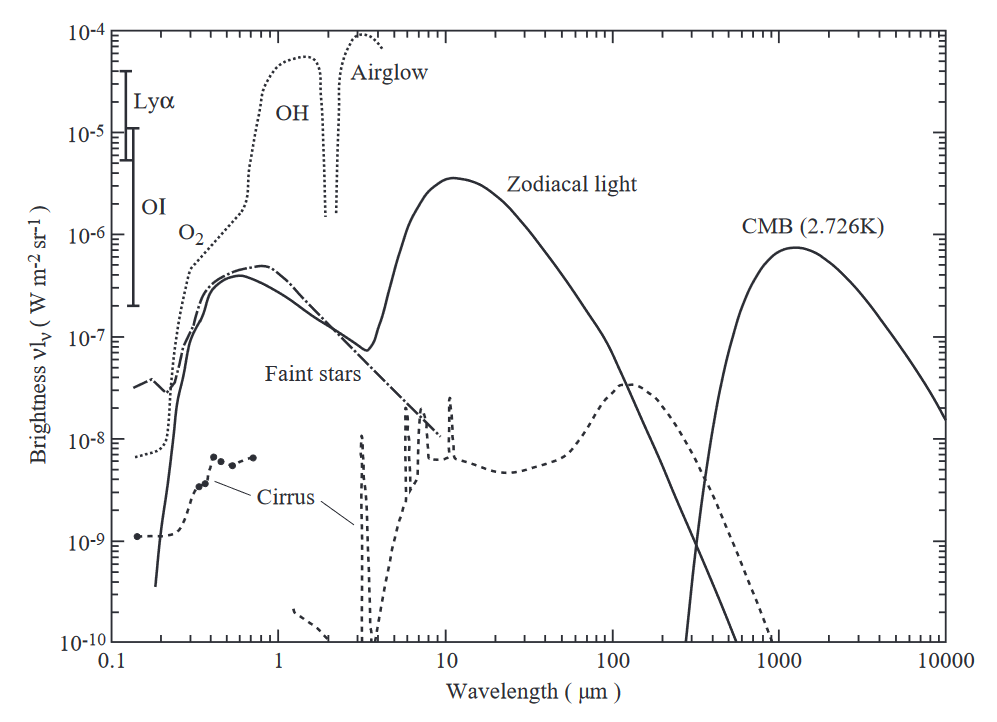
\includegraphics[width=.7\textwidth]{./2_natural_sky/natural_sources}
	\caption{Different sky brightness contributions in different electromagnetic domains. In the optical band most relevant contribution ar Airglow, zodiacal light and faint stars. From \cite{leinert19981997}.\label{fig:natural_sources}}
\end{figure}
For clarity I will distinguish between extraterrestrial sources from the terrestrial or atmospheric ones. At the end of the chapter I will also discuss about the contribution on the sky background due to atmospheric scattering effects.

Quantitatively the total sky brightness can be expressed as
\begin{equation}
	I_\text{sky} = (I_A+I_{ZL}+I_{ISL}+I_{DGL}+I_{EBL})e^{-\tau}+I_\text{sca}
\end{equation}
where A stands for airglow, EZ is zodiacal light, ISL integrated galactic light, DGL diffuse galactic light and EBL extragalactic background light. $\tau$ is the extinction coefficients and $I_\text{sca}$ gathers all the scattering terms, i.e.\ light scattered from previous sources and from light pollution, from \cite{leinert19981997}.


\section{Extraterrestrial sources}
I will first consider sources of photons outside the earth atmosphere. Using space-based instrument it is possible to study these components without the interference of atmospheric emissions.

\subsection{Zodiacal light}
Zodiacal light consists on sunlight scattered by interplanetary dust particles \cite{leinert1975zodiacal}. From the Earth it looks like a white glow visible during the twilight and extending from the Sun in the zodiacal region.
\begin{figure}
	\centering
	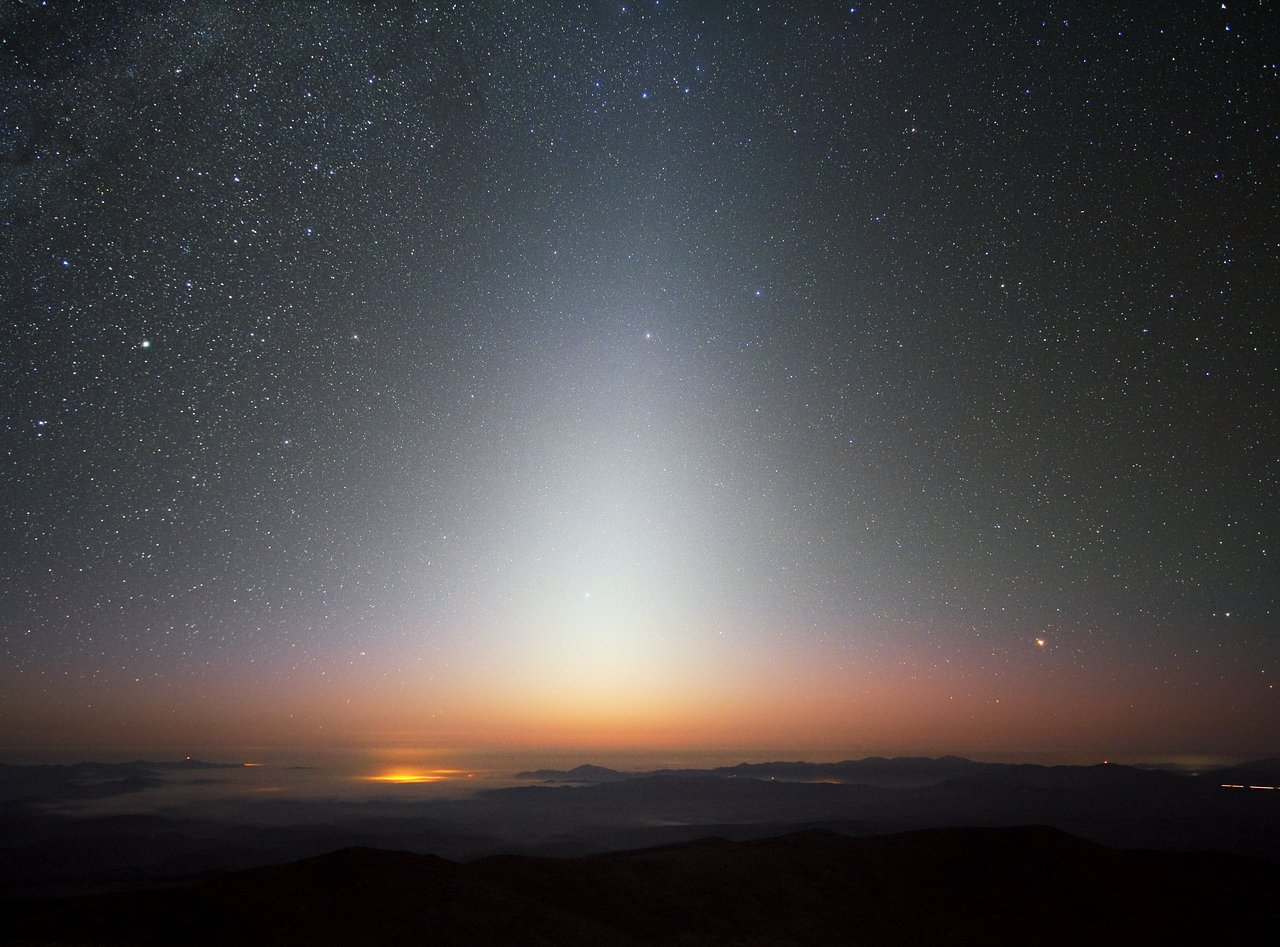
\includegraphics[width=.8\textwidth]{./2_natural_sky/zodiacal_ima}
	\caption{Zodiacal light after sunset at La Silla, Chile. Source: \href{https://www.eso.org/public/images/zodiacal_beletsky_potw/}{eso.org}.\label{fig:zodiacal_ima}}
\end{figure}

\paragraph{Angular distribution.} The figure \ref{fig:zodiacal_distribution}, adapted from \cite{frey1974photometry}, describes the angular distribution of the zodiacal light in ecliptic coordinates. Such light is maximum along the ecliptic and close to the Sun. A fainter local maximum is present in direction opposite to the Sun. It is known as \emph{gegenschein} and is produced by back-scattered solar light. Zodiacal light brightness varies from about \SI{e-6}{erg\per\second \per\centi\metre\squared \per\steradian\per\angstrom} on the ecliptic at \ang{30} from the sun to about \SI{e-9}{erg\per\second \per\centi\metre\squared \per\steradian\per\angstrom}. Gegenschein maximum brightness reaches about \SI{e-7}{erg\per\second \per\centi\metre\squared \per\steradian\per\angstrom}. After the airglow (see \S XX), this is the second brightest background source in optical bands.

\begin{figure}
	\centering
	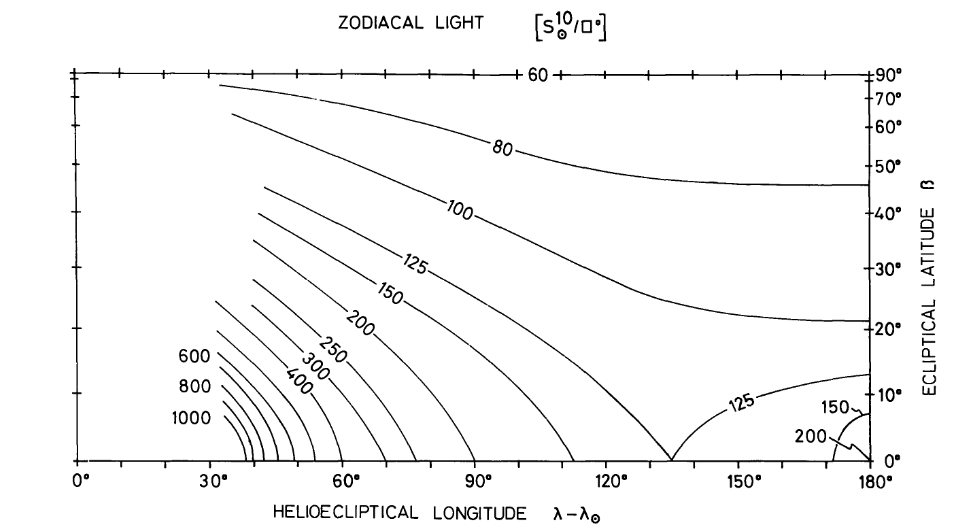
\includegraphics[width=.8\textwidth]{./2_natural_sky/zodiacal_distribution}
	\caption{Isophotal map ot the zodiacal light as \SI{7100}{\angstrom}. As a reference, according to \cite{leinert19981997}, $\SI{1}{S}_{10}/\square^\circ = \SI{9.21e-10}{erg\per\second \per\centi\metre\squared \per\steradian\per\angstrom}$ at those wavelengths. From \cite{frey1974photometry}.\label{fig:zodiacal_distribution}}
\end{figure}

The contribution of zodiacal light to the optical background is maximum during the twilight, after sunset in spring or before sunrise in autumn, from the northern hemisphere.

\paragraph{Spectral energy distribution.} Being essentially reflected sunlight, the optical zodiacal light energy distribution has the same shape of the solar one.

\subsection{Galactic background}
In optical bands a significant contribution to the background level is provided by unresolved stars in the Galaxy. The contribution of such sources depends on the ability of resolve the brightest stars \cite{leinert19981997}, i.e.\ on the limiting magnitude of the instrument.

\paragraph{Angular distribution.} Unresolved stars background follows the morphological structure of the Milky Way. The signal is higher toward the galactic plane and the galactic center.  Its spectrum follows typical optical stellar spectra with the characteristic black-body emission. It is the third most relevant contribution to the optic continuum with an emission that spans from peak values of \SI{e-6}{erg\per\second \per\centi\metre\squared \per\steradian\per\angstrom} in the most crowded areas to \SI{e-8}{erg\per\second \per\centi\metre\squared \per\steradian\per\angstrom} toward the galactic poles.

\subsection{Diffuse galactic light}
Similar to the zodiacal light, it is the result of the scattering of stellar emission with interstellar dust particles. \cite{leinert19981997} estimate its contribution as between 20\% and 30\% of the total integrated light from the galaxy. This estimation is rather uncertain because of the faintness of the radiation and the contamination of direct stellar light. There are no comprehensive maps for the diffuse galactic light but it is very likely this emission to be concentrated along the galactic disk, analogously to the direct stellar component. Its spectral energy distribution is comparable with stellar spectra, since its nature of stellar reflected light.

\subsection{Extragalactic background}
A much smaller contribution is led by the extragalactic background, i.e.\ emission of faint and or unresolved galaxies. It is very difficult to quantify the resulting brightness and in many cases are available only the upper limits for extragalactic background. The main estimation difficulties are due to the faintness of the signal and with respect to the other sources. Typical values of intensity are of the order \SI{e-9}{erg\per\second \per\centi\metre\squared \per\steradian\per\angstrom}. No reliable information about spatial distribution is available.

\section{Terrestrial sources}
Terrestrial sources are those capable of producing visible photons in the atmosphere.

\subsection{Airglow}
The airglow is the faint emission on the higher layers of the atmosphere, produced by the interaction between atoms and the particles from the solar wind or by the chemical interaction between atoms. High energy solar particles collide with the atmospheric atoms exciting their electrons to higher energy levels; when the electrons jump back to the initial states they release energy in form of photons, leading to the characteristic emission spectrum. Another possible emission channel is by chemical recombination: when atomic oxygen collide with nitrogen or hydrogen atoms a single molecule (NO or OH) is created and a photon is released. Atomic oxygen or nitrogen are produced by photodissociation of the respective molecules during the day by solar radiation.
\begin{figure}
	\centering
	\includegraphics[width=.8\textwidth]{./2_natural_sky/airglow}
	\caption{Oxygen (green) and sodium (orange) airglow emission, photographed from the ISS. Source: \href{https://eol.jsc.nasa.gov/SearchPhotos/photo.pl?mission=ISS043&roll=E&frame=143486}{eol.jcs.nasa.gov}.\label{fig:airglow}}
\end{figure}

\paragraph{Main components.} We can subdivide the airglow sources as a function of the height of the emitting layer. A first layer between 85 and \SI{100}{km} is provided by molecular oxygen, sodium (respectively Herzberg  bands and Fraunhofer D line) and OH transitions. Going higher, up to \SI{300}{km}, forbidden atomic oxygen lines are produced. The outermost layers of the atmosphere, above \SI{1000}{km}, are usually referred as geocorona; is this region faint but detectable hydrogen lines are produced.

Being produced by thin and homogeneous layers, the airglow emission is relatively uniformly distributed in the sky sphere, with an increase of brightness at high zenital distances due to the increase of geometric depth along the line of sight. Maximum brightness is achieved at about \ang{10} above the horizon after that the overall brightness is dimmed by atmospheric extinction. Brightest lines can produce a brightness up to \SI{e-5}{erg\per\second \per\centi\metre\squared \per\steradian\per\angstrom}

\paragraph{Variations in airglow emission.} Airglow emission varies in time, both on short and long timescales, following the behavior of the atmosphere and the solar activity \cite{leinert19981997}. Emission is also related to the geomagnetic latitude: is maximal in the sub-polar region, at a latitude of about $\ang{60}-\ang{80}$ after which it significantly drop. In the polar region airglow emissions are substituted with auroral emission. In the low latitude regions emissions are generally low with a slight increase toward the equator \cite{eather1969latitudinal}.

\subsection{Aurorae}
Aurorae are bright light bands observable at polar latitudes. They are produced by the excitation of atoms in the high layers of the atmosphere by the solar wind. At high latitudes interplanetary high energy charged particles can penetrate the magnetosphere ad reach the atmosphere where they collide and excite atmospheric elements. Excitation energy is then released in form of a photon, responsible for the observed radiation. Auroral spectrum is constituted by emission lines. Colors ranges from green and orange (typical of oxygen transitions) to blue or purple (trace of nitrogen emission), see figure \ref{fig:aurora}.
\begin{figure}
	\centering
	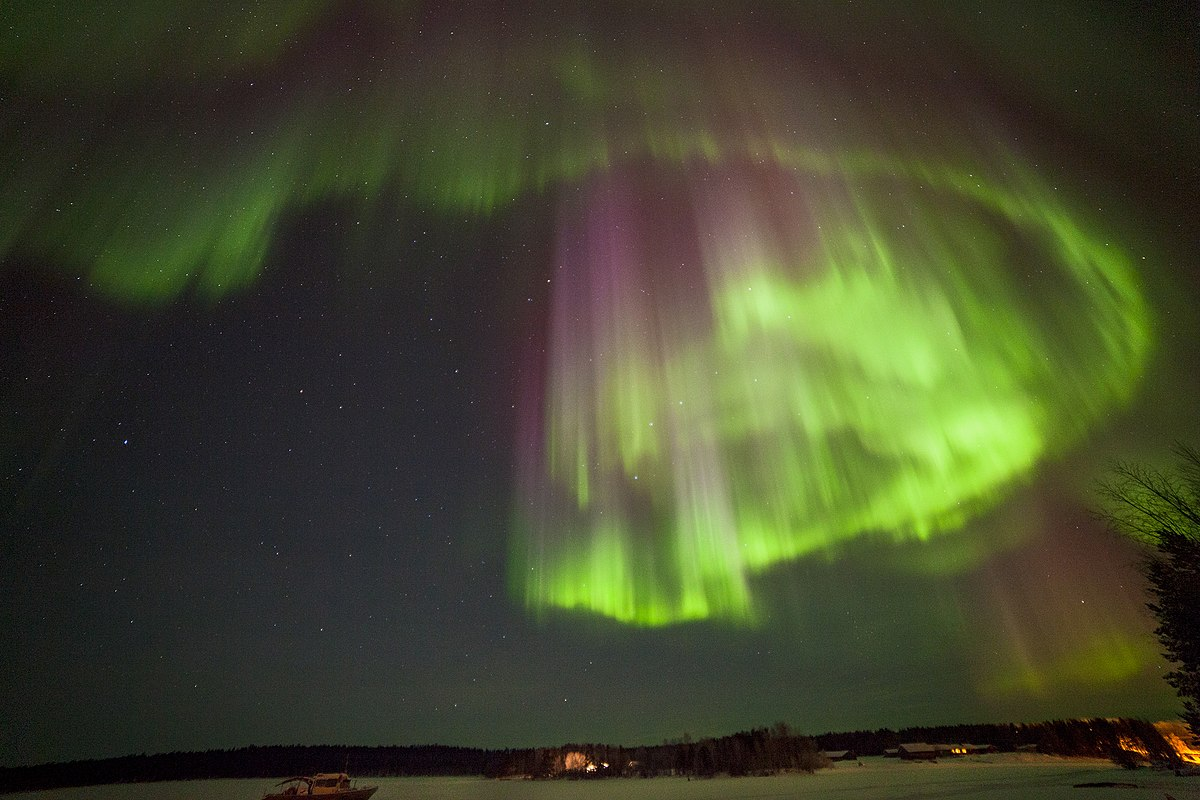
\includegraphics[width=.8\textwidth]{./2_natural_sky/aurora}
	\caption{Aurora borealis in the northern Finland. Credits: \href{https://commons.wikimedia.org/wiki/File:Aurora_Borealis_-_polar_lights_3.jpg}{Martincco}.\label{fig:aurora}}
\end{figure}

The occurrence and intensity of this phenomenon is strictly regulated by the solar activity, and an increase of auroral emission can be observed during solar storms or period of high activity. The phenomenon is observable only in polar regions, namely above \ang{80} of latitude (see \cite{eather1969latitudinal}) and for this reason it has a limited impact on the total optical sky background only in that geographic area. Nevertheless in case of intense solar activity like solar storms, aurorae can be observed at lower latitudes. Historical sources even report the sporadic observation of aurorae up to temperate latitudes.


\section{Atmospheric scattering}
Atmospheric scattering refers to the interaction of light with aerosol particles in the atmosphere. Unlike reflection or refraction, when a light beam get scattered its photons are deflected in random directions. In the Earth atmosphere the main aerosol particles are XXXXX.

\subsection{Scattering mechanisms}
There are two main scattering mechanism, depending on the size of the particle with respect to the wavelength of the incident radiation: Mie and Rayleigh scattering.

\paragraph{Mie scattering.}

\paragraph{Rayleigh scattering.}

\subsection{Effects on the sky brightness}
Every light source is responsible for a certain amount of light scattering. Depending on the site and the observation time, the effects of scattering on the total sky brightness can vary significantly.

\paragraph{Dark sites.} In a dark site most of the scattered light is produced by airglow, zodiacal light and the galactic background, i.e.\ the brightest ``direct'' light sources. According to \cite{leinert19981997} scattered light from the natural sources accounts for a brightness of the order of \num{e-8} to \SI{e-7}{erg\per\second \per\centi\metre\squared \per\steradian\per\angstrom}.

\paragraph{Light polluted sites.} Atmospheric light scattering is the main mechanism responsible for light pollution when far from the light source. Due to Earth curvature, geographic features and atmospheric extinction the direct light contribute to pollution only when very close to the light source. As reported in the chapter XX, brightness of scattered artificial light from a city varies with the population and the distance.

\paragraph{Scattered sunlight and moonlight.} Scattering is responsible for the twilight: even if the Sun is below the horizon some residual scattered light still brightens the sky. Conventionally astronomical twilight ends when the sun is \ang{18} below the horizon and other light sources, such as zodiacal light, becomes more relevant.

A similar effect is provided by scattered moonlight. Such light brightness depends on the lunar phase and on the distance between the Moon and the observing position in the sky. According to \cite{krisciunas1991model} and similar sources, in optical bands scattered moonlight can lead to an increase of the sky brightness of the order of \SI{5}{mag\per {arcsec}\squared}.
\chapter{Artificial sky light pollution}
\chapter{The spectrum of the sky}
\chapter{Sky spectra reduction}

In this chapter are reported the steps in the data reduction that I designed to extract spectra of the sky from frames originally taken for scientific purposes. After a brief overview I describe accurately the data reduction process that I built. To improve the readability of this writing, I will report only the most significant pieces of code.

\section{Introduction}

\subsection{Software management and reduction steps}
In this work I developed some pieces of Python (v.\ 3.10) code to manage all the steps of the data reduction. Note that most of the data pre-reduction was already done and was not necessary to use old software such as IRAF or its python version PyRAF. In this work I tried to heavily automatize the script in order to be able to analyze all the frames with a single run. Many efforts were spent to build a robust code, capable of working correctly for spectra with very different features, without the necessity to fine-tune the software settings every single time a new frame is processed. All of this effort was made in order to be eventually able, in the future, to rapidly analyze new frames.

I decided to divide the source code into different independent scripts, each one devoted to a specific task. It follows a brief description of each step of the data reduction process.
\begin{description}
	\item [Background extraction] Starting from the original spectra I have to separate the scientific targets from the background regions. Once identified the spectra of the targets and the cosmic rays, the relative regions are masked. The remaining area contains the spectrum from the sky background only and is extracted to a new file.
	\item [Background analysis] The sky spectrum is averaged along the slit direction. From the regions that do not present lines is estimated the shape of the sky continuum emission. Prominent lines or lines of interest are identified and the relative equivalent width is computed. The output of background analysis is the estimation of the continuum emission and the list of the widths of the emission lines.
	\item [Line analysis] The width of the same line is compared in the different frames. Particular attention is devoted to the line intensity with the epoch of observation and the direction in the sky.
	\item [Continuum analysis] Continuum intensity in different bands of the spectra is computed and correlated again with the epoch and direction of observation.
\end{description}

\subsection{The dataset}
This work is based on 35 spectra taken between 2006 and 2020 in the Osservatorio Astrofisico di Asiago, Asiago, northern Italy. Spectra were collected by professor Stefano Ciroi and collaborators to collect data on studied astronomical objects and were taken with the \SI{1.22}{m} reflective telescope ``Galileo Galilei'' equipped with the grating spectrograph ``Boller\&Chivens''.

Each frame has been pre-reduced by Ciroi and its work group: data has been corrected for bias and flat field and calibration on both flux and wavelength was performed. Cosmic rays were not removed as well as the sky background. Before November 2011 frames had a spatial scale on the CCD of \SI{0.63}{arcsec\per{px}} while on later data the scale was \SI{1.0}{arcsec\per{px}}. For all the object, grating with a line density of \SI{300}{tr\per{mm}} was used while the grating angle varied between \ang{0} and \ang{5.25} according to the type of target. Similarly slit aperture size varied from a minimum of 200 to a maximum of \SI{400}{\micro\metre} while the exposure times ranged between 300 and \SI{3600}{s}.

\section{Background extraction}
The data available was not taken with the aim of monitoring the sky condition and thus contain astronomical objects. The first step in the data reduction is to identify the regions of the spectra where there are the scientific targets. Most of the effort described below is to automate the process.

On the figure \ref{fig:raw_spec} is shown as an example the spectrum obtained in the 6 November 2020 pointing at the active galaxy labeled 4FGL J0512. Two main astronomical sources are visible as long strips in the top and bottom side of the frame. The other bright vertical lines and bands represent the emission of the sky diffuse background. Looking carefully some cosmic rays can be also spotted toward bluer wavelengths. This frame will be used later to show the different steps in the data process.

\begin{figure}[h!]
	\centering
	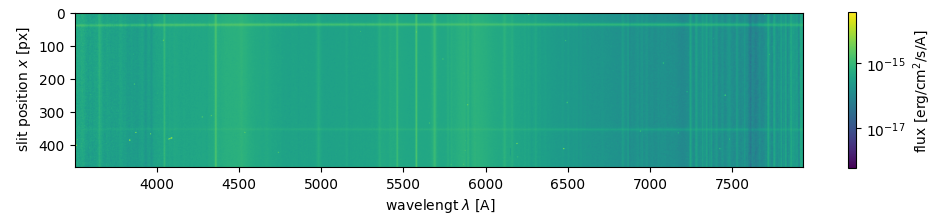
\includegraphics[width=\textwidth]{./5_mywork/raw_spec}
	\caption{An example spectrum from the dataset. The frame contains the active galaxy ``4FGL J0152''. Main components are the galaxy and another source (horizontal stripes), the diffuse background (vertical lines and bands) and some cosmic rays (especially below \SI{4000}{\angstrom}).\label{fig:raw_spec}}
\end{figure}

\subsection{Preamble}
Before the actual data analysis I need to load all the necessary.

\paragraph{Modules, options and parameters.}
First I need to load packages and set parameters to allow the rest of the script to work correctly.
\begin{lstlisting}
import numpy as np
import matplotlib.pyplot as plt
from astropy.io import fits
from scipy.signal import find_peaks, peak_widths
from datetime import datetime
import glob
import os
from wotan import flatten
from scipy.optimize import curve_fit

######################
#OPTIONS
save_plots = True
save_FITS = False
plot_profile = True
plot_spec = True
show_ima = False

#PARAMS
peak_height = 0.05 #height abouve the bkg level
data_col_frac = .75 #minimum fraction of valid pixels in a column
width_mult = 2 # interval to exclude around a source, wrt center in FWHM units
cr_width = 2.5 # cr trace spatial width
cr_prominence = 5 #treshold height wrt average column level
cr_pad = 1 # number of px to exclude around cr, in a fixed column
LAMBDA_lim = 3500 #A, limit blue wavelength
######################
\end{lstlisting}
Options are some special parameters that allow to enable or disable some debugging diagnostics useful in the development phase. Parameters are some special values that can be changed to control the final output result. Each of these lines will be explained later when appearing in the code.

\paragraph{Data import and handling.} Each spectrum is stored in a \texttt{.fits} file (acronym of Flexible Image Transport System, see \nota{biblio FITS format}). For this work I need both the actual spectrum data and the auxiliary information about the acquisition and reduction processes, contained in the header section.

To automate the process of data import I used the \texttt{glob} function from the homonyms module (\nota{citare glob package}) to identify all the files with the FITS extension in a given path directory. I also needed the function \texttt{basename} from the \texttt{os.path} module (\nota{citare os.path}) to retrieve the actual name of each file, since \texttt{glob.glob} provides only the full path of the files. Then the file research is implemented with the following code.
\begin{lstlisting}
#browse all the *.fc.fits files in a directory and its subdirectories
main_path = './Asiago_nightsky/'
file_ls = glob.glob(main_path+'/**/*.fc.fits', recursive= True)
names = [os.path.basename(x) for x in file_ls]
\end{lstlisting}
\texttt{main\_path} can be eventually adapted to scan new files in different directories. The choice to search for files that ends with \texttt{.fc.fits} is due to the fact that Ciroi and collaborators use the convention to append the suffixes \texttt{.f} and \texttt{.c} to indicate frames corrected for flat field and calibrated respectively.

\subsection{Data extraction}
For each file found in the \texttt{main\_path} directory I need to extract the information contained both in the header and the data unit(s). This task is performed by the \texttt{astropy.fits.io} module and is implemented in the following way:
\begin{lstlisting}
#process all the files found
for name,file in zip(names,file_ls):

	#open a FITS file
	hdul = fits.open(file)
	hdr = hdul[0].header
\end{lstlisting}
The header is a Python dictionary from which I can extract the quantities that I will need as new variables.

\paragraph{Wavelength data.} The first thing to extract is the wavelength information in the following way.
\begin{lstlisting}
	#extract wavelenght information from the header
	NAXIS1, NAXIS2 = hdr['NAXIS1'], hdr['NAXIS2']
	LAMBDA0, DELTA = hdr['CRVAL1'], hdr['CDELT1']
	
	#generate the lambdas array
	if hdr['CTYPE1'] != 'LINEAR':
		print('WARNING: no linear wavelength calibration')    
	LAMBDA = np.arange(LAMBDA0, LAMBDA0+NAXIS1*DELTA, DELTA)
	if len(LAMBDA) == NAXIS1+1:
		LAMBDA = LAMBDA[:-1]
	
	#remove extreme blue wavelengths
	LAMBDA_start_id = len(LAMBDA)-len(LAMBDA[ LAMBDA>LAMBDA_lim])
	LAMBDA = LAMBDA[LAMBDA_start_id:]
\end{lstlisting}
In this way the array \texttt{LAMBDA} contains the wavelength associated to each column of the spectrum, assuming a linear calibration. In the case the original calibration is not linear, a warning message is printed.

I decided to limit the wavelengths in the blue hand of the spectrum to the limit value \texttt{LAMBDA\_lim} which was set to \SI{3500}{\angstrom}. Below this threshold the signal tends to be too noisy and low quality, due to the strong correction in the flux calibration phase and the intrinsic low sensitivity of CCDs in the blue domain. Also \texttt{LAMBDA\_lim} is meant to be a parameter that can eventually be changed to fit new data.

In the figure \ref{fig:10_det} is show the bluest hand of the spectrum of the planetary nebula NGC2392 (also known as ``The Eskimo nebula''), taken on the 1 February 2006: the signal is extremely noisy due to the extreme calibration necessary at those wavelengths. Note also the presence of several cosmic rays (red circles) that provide further spurious signals to the spectrum.
\begin{figure}[h!]
	\centering
	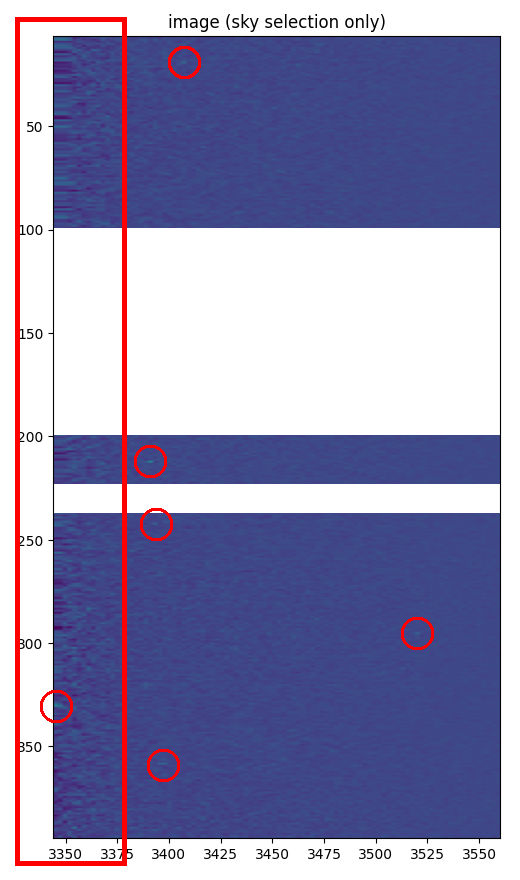
\includegraphics[width=.4\textwidth,angle=90]{./5_mywork/10_det}
	\caption{Extreme blue/UV domain in the spectrum of the nebula NGC2392. The area in the rectangle is totally useless due to the noise. Cosmic rays have been highlighted too. \label{fig:10_det}}
\end{figure}

\paragraph{Slit and scale data.} For my script I will also need information about the angular scale of the spectra. In particular I want to retrieve the angular scale on the final spectrum (in arcsec/px) and the size of the slit on the detector (in px). Implementation is the following:
\begin{lstlisting}	
	year = hdr['DATE-OBS'][:4]
	
	#aperture information from the hdr
	SLIT = hdr['SLIT'] #microns
	try:
		BINX, BINY = hdr['BINX'], hdr['BINY'] #binning factors
		TELSCALE = hdr['TELSCALE'] #arcsec/mm
		CCDSCALE = hdr['CCDSCALE'] #arcsec/px
	except KeyError:
		BINX, BINY = hdr['HBIN'], hdr['VBIN']
	
		print(' WARNING: no scale info in the hdr (using defauls)')
	
		TELSCALE = 10.70 #arcsec/mm #TO BE CHECKED!!!
		CCDSCALE = 0.63 #arcsec/px #TO BE CHECKED!!!
	
	SLIT_angular = SLIT/1000 * TELSCALE #slit size in arcsec
	SLIT_px = SLIT_angular / CCDSCALE / BINX #slit size in px
\end{lstlisting}
Note the \texttt{TELSCALE} and \texttt{CCDSCALE} entries in the file header are available only from 2009. For earlier files I had to set by hand these two variables; in this case a warning message is also displayed. As reported in the code, as stated in \nota{citare proprietà CCD prima del 2009} before 2009 the telescope scale was of \SI{10.70}{arcsec\per{mm}} while the scale on the detector was \SI{0.63}{arcsec\per{px}}.

\subsection{Cosmic ray and noise removal}
The next step in the sky extraction process is to remove the cosmic rays and the residual noise in the blue domain. These two sources of photons provide spurious signals that may interfere with the detection and removal of the astronomical signal from the background. See for example the figure \ref{fig:10_det} at page \pageref{fig:10_det}.

Implementing an automatic process of recognition and masking of the spurious signals from cosmic rays and photon noise is rather complex and requires quite advanced analysis tools. The steps I made are the following:
\begin{enumerate}
	\item I scan each column of the spectrum, i.e.\ for each fixed value of the wavelength. The average flux level of the column is computed as a reference of the brightness of the spectrum at the analyzed wavelength.
	\item In each column I look for sharp peaks in the flux due to the presence of cosmic rays or strong noise. The peaks are identified with the function \texttt{find peaks} from the module \texttt{scipy.signal}. In particular I restricted only to peaks with a width below the value of \texttt{cr\_width}$=\SI{2.5}{px}$ and a prominence\footnote{\nota{info prominence significato}} higher than \texttt{cr\_prominence}$=5$ times the average value of the column. These are good settings to filter only peaks of noise and cosmic rays that are typically very sharp and much brighter than the astronomical signal.
	\item I mask the pixels around the peaks. The number of pixels to mask is computed from the width of the peaks, which is provided by the function \texttt{peak\_widths} from the module \texttt{scipy.signal}. I used this function to compute the FWHM of each peak, since this was a more solid width estimator with respect to the full width, which may be biased due to the noise fluctuations around the peak. I assumed that the total width of the peak was $2\times\text{FWHM}$. To be sure all the cosmic rays traces or the noise fluctuations were contained in the detected width, I conservatively decided to increase the masked interval of a further \texttt{cr\_pad}$=\SI{1}{px}$ in both directions along the columns.
	\item I remove all the columns where too many pixels have been masked, i.e.\ too noisy columns. The minimum fraction of saved pixels in a column must be higher than the value \texttt{data\_col\_frac}$=0.75$.	
\end{enumerate}
After the removal of sharp peaks and noisy columns I expect to have a clean frame which contains only the spectra of the astronomical targets and the background sky. The procedure described above is implemented by the following lines.
\begin{lstlisting}
	######################
	#bkg level estiamtion
	raw_data = hdul[0].data[:,LAMBDA_start_id:]
	raw_integr = np.sum(raw_data, axis = 1)
	bkg_est = np.nanmedian(raw_integr)  
	
	######################
	#remove cosmic rays and UV noise
	x = np.arange(len(raw_integr)) 
	data = np.copy(raw_data)
	
	cr_col_frac = np.zeros(len(LAMBDA)) #fraction of remaining px
	for cr_col,col in enumerate(data.T):
		col_avg = np.nanmean(data[:,cr_col])
		cr_line,_ = find_peaks(col,
							   prominence = cr_prominence*col_avg,
							   width = (0,cr_width))
	
		cr_widths = peak_widths(col, cr_line, rel_height=0.5)[0]
	
		#set left and right boundaries of the source region along the slit
		left_width = cr_line-cr_widths - cr_pad
		right_width = cr_line+cr_widths + cr_pad
	
		#scan each column and remove peaks
		cr_sel = np.zeros(np.shape(col), dtype=bool)
		for i in range(np.shape(col)[0]):
			for peak,width in zip(cr_line,cr_widths):
				if abs(i-peak) < width+cr_pad:
					cr_sel[i] = True
	
		#counts how many pixels are left in a column
		saved_px = (NAXIS2 - np.sum(cr_sel))/NAXIS2
		cr_col_frac[cr_col] = saved_px
		if saved_px >= data_col_frac: #if enough, take the masked column
			data[cr_sel, cr_col] = np.nan
		else: #else discart the entire column
			data[:, cr_col] = 0.
\end{lstlisting}


%%%%%%%%%%%%%%%%%%%%%%%%%%%%%%%%%%%%%%%%%%%%%%%%%
%fine controllo ortografico
%%%%%%%%%%%%%%%%%%%%%%%%%%%%%%%%%%%%%%%%%%%%%%%%%

\subsection{Sources identification}
The main idea to find scientific target is to integrate the (cleaned) spectrum in the wavelenghts and obtain the integrated luminosity profile of telescope field through the slit. Astromical sources are spatially limited and thus appear as bright peaks over the flat homogeneus background. Unluckyly in some real spectra the continuum is not homogeneus but present some gradients, probably due to some calibration biases; consequently the background integrated luminosity profile may not be flat at all, complicating the detection of astrnomical signals. If $F(x)$ is the total luminosity profile, we can imagine to split the two components
\begin{equation}
	F(x)=A(x)+B(x)
\end{equation}
where $A$ is the signal due to the astronomical sources and $B$ the one from the background.

The full implementation of the identification process follows the steps below:
\begin{enumerate}
	\item Integrate the spectrum along the wavelengths to retrieve the luminosity profile along the slit. Estimate the typical luminosity value of each profile as the median one; median value is much less sensitive to peaks in the luminosity profile and for this reason is preferable with respect to other estimations such as the average.
	
	If $F(x,\lambda)$ is the flux in a pixel of the spectrum in the position $x$ along the slit and wavelenght $\lambda$, then the luminosity profile $F(x)$ is obtained as
	\begin{equation}
		F(x)=\int_{\lambda_{min}}^{\lambda_{max}}F(x,\lambda')\text{d}\lambda'
	\end{equation}
	while typical luminosity value is
	\begin{equation}
		\hat F = \underset{x}{\text{median}}\large\{ F(x) \large\}
	\end{equation}
	\item Estimate the general trend of the background $B$, i.e.\ regardless the presence of peaks of the astronomical targets. I used the function \texttt{flatten} from the \texttt{wotam} package (\nota{citare wotam}) to perform a bi-weighted detrending of the signal. This technique consist on estimating the smoothened value of the signal in the position $x$ as the median value of the data centered in $x$ and a window of total span $w$. A more robust indicator is obtained when data are filtered such that points with a larger displacement to the median value are less relevant. Given the value of the residual $a$ of the data with respect to the median value, there can be several different types of relative weight functions; in the wotam package it is used the Tukey function which is expressed as
	\begin{equation}
		L(a) = \begin{cases}
		\left[-\left(\frac{a}{c}\right)^2\right]^2\quad \text{if}\ | a| < c\\
		0\qquad\qquad\quad\text{else}
		\end{cases}
	\end{equation}
	where $c$ is a tuning parameter that specifies the steepness of the weight scale.
	
	I used a windowing of 50\% the total profile length and a fine-tuning parameter \texttt{cval}$=c=10$. Such large window can only partially smooth down the peaks signals. Called $\mathcal{S}_{w,c}$ the biweighted filter operator, with window $w$ and tuning parameter $c$ then the smoothed luminosity profile is given by
	\begin{equation}
		F'(x)= \mathcal{S}_{w,c}\large\{ F(x) \large\}
	\end{equation}
	\item A better approximation for the background $B$ can be obtained by masking the data around the astronomical sources. I
	used as threshold the detrended profile $F'$, vertically shifted by a factor equal to the 5\% of the average
	bkg level $\hat F$. The new profile obtained is
	\begin{equation}
		F''(x) = F'(x)\cdot\theta(x)\qquad\text{where}\quad\theta(x)=\begin{cases}
		1\ \ \quad \text{if}\quad F(x) \leq F'(x)+0.05\cdot\hat{F}\\
		\text{nan}\quad\text{else}
		\end{cases}
	\end{equation}
	The new masked profile $F''$ is much closer to $B$ than the original profile as the contribution of astronomical sources $A$ has been drastically decreased.
	\item The final background profile estimation is obtained by a further filtering of the masked trend $F''$. I used the \texttt{flatten} function with a window of 10\% the profile length. This allows to smooth the noise fluctuations in the background. Formally
	\begin{equation}
		B(x)\approx S_{W,c} \large\{ F''(x) \large\}
	\end{equation}
	where $W\ll w$ is the new windowing factor, while the value $c$ has been kept constant. Once estimated $B$ I can focus on the profile of the astronomical sources $A$ which can be isolated simply as $A=F-B$.
	
	In the figure \ref{fig:bkg_est} are plotted the various luminosity profiles used to retrieve the final background $B$ in my example frame (see above). In this case the background is quite contant along the slit and the signal from the sources stands out the background easily; even the preliminary filtered profile $F'$ would have been a good approximation of the background, without the necessity of further computation, which is instead necessary for frames with lower quality data.
	\begin{figure}[h!]
		\centering
		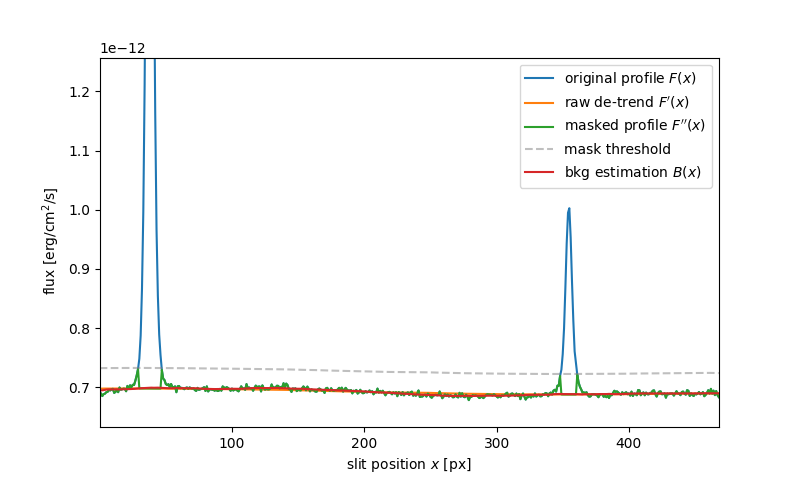
\includegraphics[width=.85\textwidth]{./5_mywork/bkg_est}
		\caption{The different luminosity profiles to estimate the background $B$ on my test frame. Thanks to the good quality of the data (uniform slit illumination, high signal-to-noise ratio) the identification of the sources is particulary easy.\label{fig:bkg_est}}
	\end{figure}

	\item Identify the peaks in the profile of the astronomical sources $A$ with the function \texttt{find\_peaks} (see above). I selected peaks higher than 5\% of the reference level $\hat F$ and broader than \texttt{cr\_width}; the first condition ensure not to include faint peaks due to background noise fluctuations, the second one, prevent from including sharp peaks produced by cosmic rays.
	\item Estimate the width of the peaks with \texttt{peak\_widths} that provided the FWHM. Many astronomical sources such as galaxies or planetary nebulae present a bright core and faint extended wings. This means that the FWHM can underestimete the total widht of a peak if wings are very broad. In a conservative approach I decided to assume the peak width as $2\times$\texttt{width\_mult}$\times\text{FWHM}$ where \texttt{width\_mult}$=2$ is another tunable parameter of the script. With the resulting widhts I masked the regions centered around the peaks.
	
	In the figure \ref{fig:removed} are shown the areas associated with the astronomical sources that has been removed, in my example frame (red bands) and the final background signal (greed dots).
	\begin{figure}[h!]
		\centering
		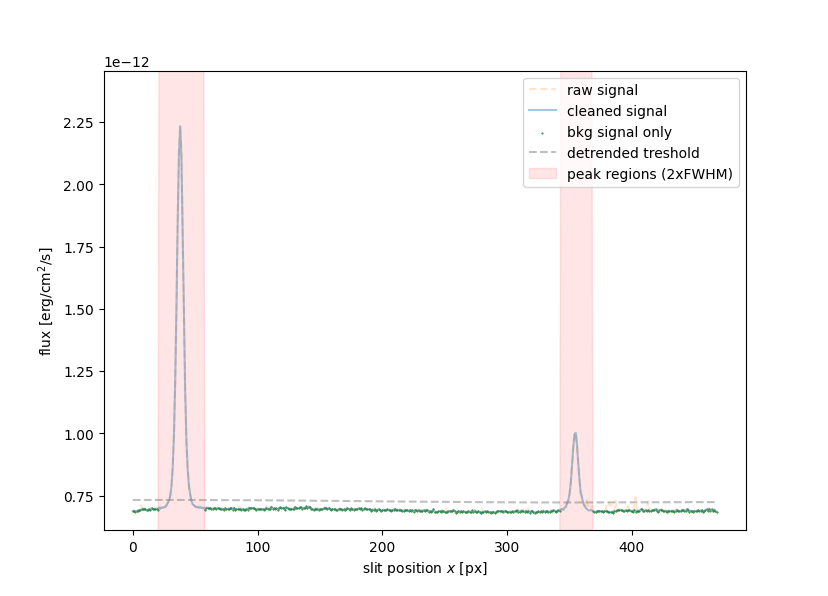
\includegraphics[width=.85\textwidth]{./5_mywork/removed}
		\caption{The astronomical sources identified by the script in the test frame. The original profile (broken orange line) has been filtered to remove cosmic rays and noise, contrinuting to smooth out the profile into the cleaned one (blue solid line). Red areas on the cleaned profile are the regions occupied by the sources and are going to be masked. The remaining usable signal from the background is represented by the green dots, each one representing a row in the bidimensional spectrum. \label{fig:removed}}
	\end{figure}
\end{enumerate}
The masked intervals in the luminosity profiles becomes masked rows, when back to the bidimensional spectrum, which should now have only counts from the sky backgorund.

On the figure \ref{fig:clean_spec} is finally reported the background sky spectrum extracted from the example frame. The white areas have been masked due to the presence of astronomical sources or cosmic rays.
\begin{figure}[h!]
	\centering
	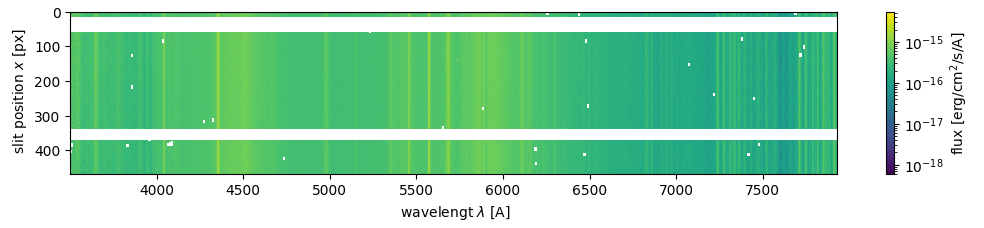
\includegraphics[width=\textwidth]{./5_mywork/clean_spec}
	\caption{Final background spectrum extracted from the example frame.\label{fig:clean_spec}}
\end{figure}


The full code to implement source extraction is the following.
\begin{lstlisting}
	#use noise/bkg info to find peaks
	integr = np.nansum(data, axis = 1)
	bkg_est = np.median(integr)
	
	#detrend: global trend (including peaks)
	_,trend_raw = flatten (x,
	                       integr ,
	                       method ='biweight',
   	                       window_length =0.5*NAXIS2 ,
	                       cval = 10, return_trend = True )
	
	#trim removing peaks, i.e. data fare above the global trend
	integr_trim = np.where(integr <= trend_raw+0.05*bkg_est,
	                       integr, trend_raw)
	
	#detrend the trimmed data, much less sensitive to the peaks
	_,trend = flatten (x,
	                   integr_trim ,
	                   method ='biweight',
	                   window_length =NAXIS/10. ,
	                   cval = 10, return_trend = True )
	
	#detrend residuals: original peaks are highlighted wrt the bkg profile
	diff = integr-trend
	
	#find peaks
	peaks,properties = find_peaks(diff, height=0.05*bkg_est, width = cr_width)
	peak_FWHM = peak_widths(integr, peaks, rel_height=.5)[0]/2.
	
	if len(peak_FWHM)== 0:
	print( " WARNING: no sources were detected")
	
	#generate a boolean mask True outside the peaks
	bkg_sel = np.full(np.shape(x), True)
	for i,peak in enumerate(peaks):
		width = (int(peak_FWHM[i])+1)*width_mult
		for w in range(-width,width):
			bkg_sel[peak+w]=False
		w = width -1
		while integr[peak+w] >= trend[peak+w]:
			bkg_sel[peak+w] = False
			w += 1
		w = width
		while integr[peak-w] >=trend[peak-w]:
			bkg_sel[peak-w]=False
			w += 1
	
	######################
	#integrated spectrum (along the slit)
	total = np.nanmean(data, axis = 0) #integration along the slit
	sky = np.nanmean(data[bkg_sel,:], axis = 0) #integration of bkg rows only
	
	total[total == 0] = np.nan
	
	######################
	#extract only the bkg rows
	
	ma_data = data #set masked data
	for i,row in enumerate(bkg_sel):
		#cancel data from the source rows
		if row == 0:
			ma_data[i,:] = np.nan
\end{lstlisting}





\subsection{Sky spectrum export}
Once masked all the contaminants, I can extract the sky spectrum and save it for further analysis. For each frame I create a new \texttt{.fits} file that contain the sky spectrum and the masked data from other sources. The header of the new file contain the same information of the original one, plus further further additional information about the time of creation and the value of the limited wavelenght \texttt{LAMBDA\_lim} (respectively ``\texttt{BKGEXTR}'' and ``\texttt{UVLIM}''). Each file is saved in the firectory of the original one and to its name is appended the \texttt{.bkg.} suffix.

\begin{lstlisting}
	######################
	#save masked data in a new FITS file
	if 1 == save_FITS:
		now = datetime.now()
		now_str = now.strftime("%Y-%m-%d %H:%M:%S")
	
		hdr.set('BKGEXTR', now_str, 'Time of bkg extraction')
		hdr.set('UVLIM', LAMBDA_lim, 'A')
		hdr['NAXIS1']=len(data[0])
		new_hdu = fits.PrimaryHDU(ma_data)
		new_hdul = fits.HDUList([new_hdu])
		new_hdul[0].header = hdr
	
		file_new = file[:-5]+'.bkg.fits'
		new_hdul.writeto(file_new, overwrite=True)
\end{lstlisting}

\section{Background analysis}



\appendix
\chapter{Source code}\label{code}
\section{Background extraction}
\lstinputlisting[language=Python]{../bkg_extractor.py}
\section{Background analysis}
\lstinputlisting[language=Python]{../bkg_analyzer.py}

\bibliography{bibliography}
\bibliographystyle{alpha}

\end{document}